\section{Progettazione}

% Devono essere esposte le scelte progettuali operate nelle varie fasi di sviluppo dell'elaborato.

% In questa sezione devono essere documentati gli schemi di progetto relativamente all'architettura complessiva del sistema e alle sue componenti di rilievo.
% Per le componenti software si può ricorrere ad esempio a diagrammi delle classi, di sequenza, stato, attività.
% Per le componenti hardware è possibile includere opportuni schemi in grado di descrivere l'architettura fisica adottata.

% Vincoli circa la lunghezza della sezione (escluse didascalie, tabelle, testo nelle immagini, schemi):
% Numero minimo di battute per 2 componenti: 12000
% Numero massimo di battute per 2 componenti: 21000

In questa sezione viene presentata l'architettura generale del sistema,
partendo da come è stata derivata a partire dai requisiti raccolti, seguendo un approccio top-down:
si affronterà quindi prima la progettazione dell'architettura ad alto livello
e in un secondo momentole effettive implementazioni e architetture di dettaglio.

Il primo passo compiuto è stata la stesura del diagramma dei casi d'uso, riportato in \Vref{fig:use-cases},
\unsure{Sarà una ripetizione con quanto dico dopo?}
fondamentale per inquadrare correttamente le funzionalità da realizzare sulla base dei requisiti.

\subsection{Architettura generale del sistema}

Come detto, il punto di partenza per l'ideazione dell'architettura sono stati i casi d'uso e i requisiti non funzionali individuati in fase di analisi:
da questi ultimi emergeva infatti la necessità di creare un sistema distribuito, scalabile e allo stesso tempo di semplice accesso.

Fin da subito, è apparsa evidente l'esigenza di implementare un'architettura che potesse distinguere livello principali:

\begin{enumerate}
  \item
    un primo livello dovrebbe essere quello dei \emph{sensori IoT}, diffusi nell'ambiente (ad esempio, almeno uno per stanza);
    essi dovrebbero svolgere al massimo una minima elaborazione locale,
    in quanto appoggiarsi al livello successivo, computazionalmente più potente, permetterebbe una maggiore flessibilità sull'analisi dei dati raccolti.
  \item
    un secondo livello dovrebbe essere un qualche tipo di \emph{appliance in rete locale} (ad esempio, almeno uno per struttura),
    in grado di svolgere il ruolo di raccolta dei dati e di \emph{gateway} verso l'esterno;
  \item
    un terzo livello, più esterno, che svolge un ruolo di aggregazione ulteriore, oltre a fornire l'accesso ai dati delle strutture da reti differenti.
\end{enumerate}

Quella che siamo andati a delineare è dunque un'architettura molto simile al concetto di \textbf{Fog Computing} come descritto da Cisco~\cite{CiscoSystems2016} nella teorizzazione originale.

Definita dunque questa architettura di massima, si è delineato le entità principali del sistema:

\begin{description}
  \item[Sensori IoT]
    Il primo livello citato sopra è costituito da sensori in grado di collegarsi autonomamente col gateway tramite protocollo wireless (ad esempio, WiFi 2.4GHz).
    Nel prototipo che si intende realizzare, si intende monitorare una singola stanza e verrà utilizzato un singolo sensore;
    l'ambiente di studio, infatti, ha stanze di media grandezza, che vengono coperte ``di misura'' dalle antenne embedded nel PCB di molti sensori dotati di modulo WiFi.
  \item[Server Fog] % TODO: ricorda di sostituire edge con fog ovunque
    Il secondo livello sarà realizzato tramite un PC a basso consumo (presumibilmente basato su SoC ARM) incaricato di ospitare:
    \begin{itemize}
      \item il codice di backend per svolgere il ruolo di \emph{gateway} tra i sensori e il cloud;
      \item un'interfaccia web in grado di mostrare informazioni sull'ambiente monitorato;
      \item gli eventuali server necessari all'infrastruttura per la comunicazioni dei sensori con il backend (come ad esempio un \emph{message bus} o un \emph{publish/subscribe broker}).
    \end{itemize}
  \item[Cloud]
    Il livello cloud sarà realizzato appoggiandosi a un provider in grado di offrire:
    \begin{itemize}
      \item
        un servizio PaaS per l'hosting del codice di backend,
        preferibilmente implementato nella medesima tecnologia scelta per il livello fog, al fine di massimizzare il riuso del codice.
      \item
        un servizio PaaS per l'hosting del codice di frontend web in grado di mostrare informazioni su tutti gli edifici monitorati (nel prototipo, uno solo).
      \item
        un servizio di database gestito, possibilmente ottimizzato verso un elevato I/O\@;
        per il momento, l'essere relazionale o meno non è considerato rilevante.
    \end{itemize}
\end{description}

In \Cref{fig:architecture} è riassunto graficamente quanto descirtto sopra.

\begin{figure}[H]
  \centering
  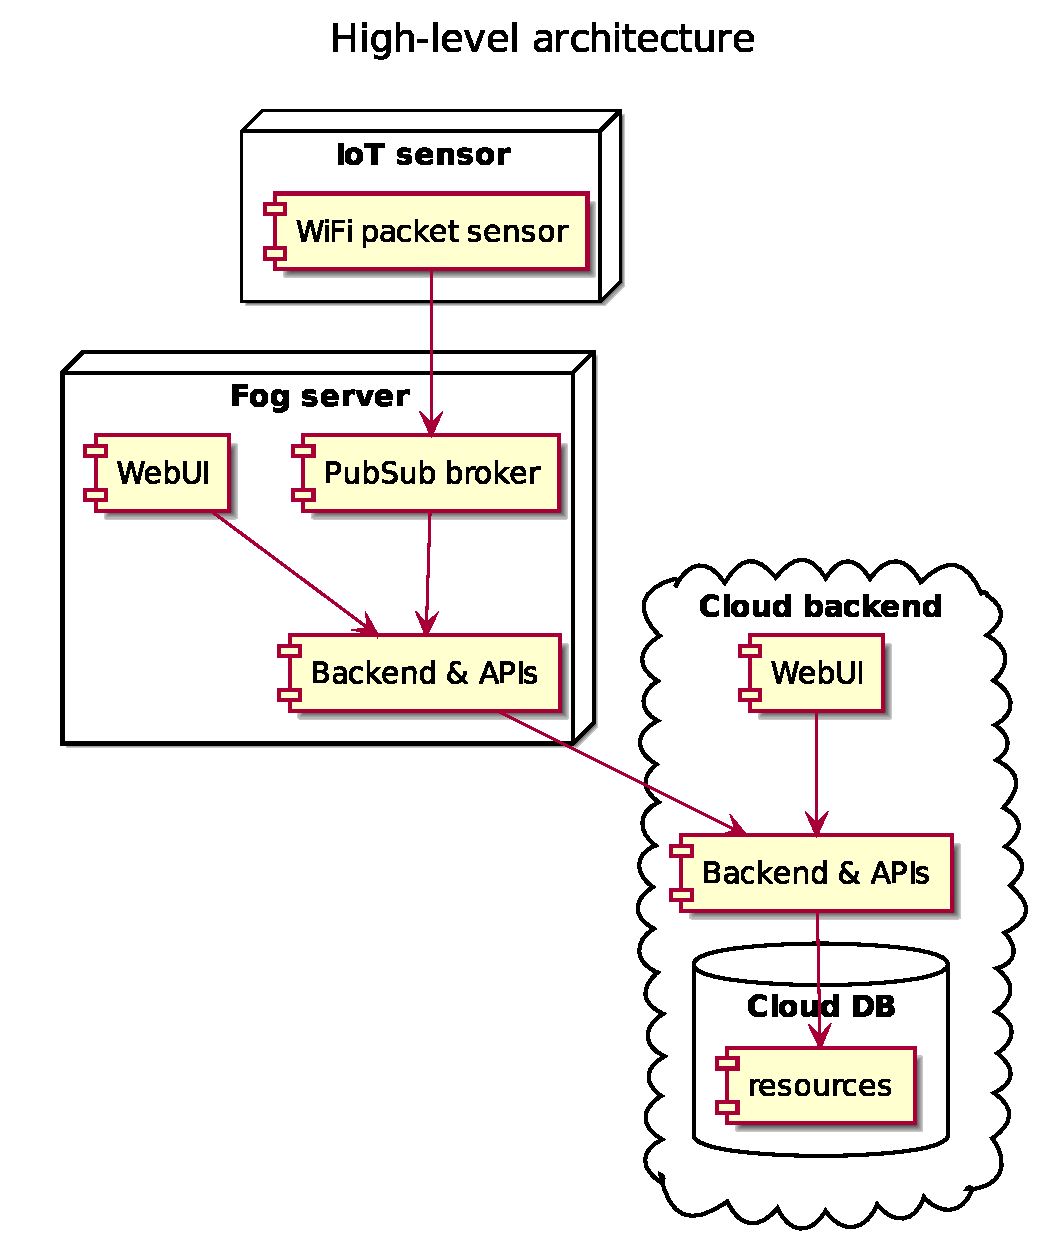
\includegraphics[width=\textwidth]{res/out/architecture.eps}
  \caption{Diagramma che riassme le componenti di massima dell'architettura del sistema}%
  \label{fig:architecture}
\end{figure}

\subsection{Interazioni tra gli elementi del sistema}

\subsection{Hardware necessario}
